\documentclass{article}
\usepackage{graphicx, amsmath}
\graphicspath{ {./images/} }

\title{HW 7.3 Solns}
\author{Principles of Microeconomics}
\date{\today}

\begin{document}

\maketitle

\subsection*{Quick Quiz}

\begin{enumerate}
\setcounter{enumi}{6}

\item (a) --
	\begin{align*}
	CS &= WTP - P \\
	&= 300 - 200 \\
	&= 100 \\
	PS &= P - Cost \\
	&= 200 - 2(60) \\
	&= 80 \\
	CS - PS &= 100 - 80 \\
	&= 20
	\end{align*}
	
\item (c) -- By definition, an efficient outcome maximizes total surplus which is the sum of consumer surplus and producer surplus.

\newpage

\item (b) -- At equilibrium, buyers and sellers are represented by the segments of the demand and supply curves to the left of equilibrium. Since those are the highest and lowest segments of the demand and supply curves respectively, the buyers and sellers are those with the highest willingnesses to pay and lowest costs.

	\begin{center}
	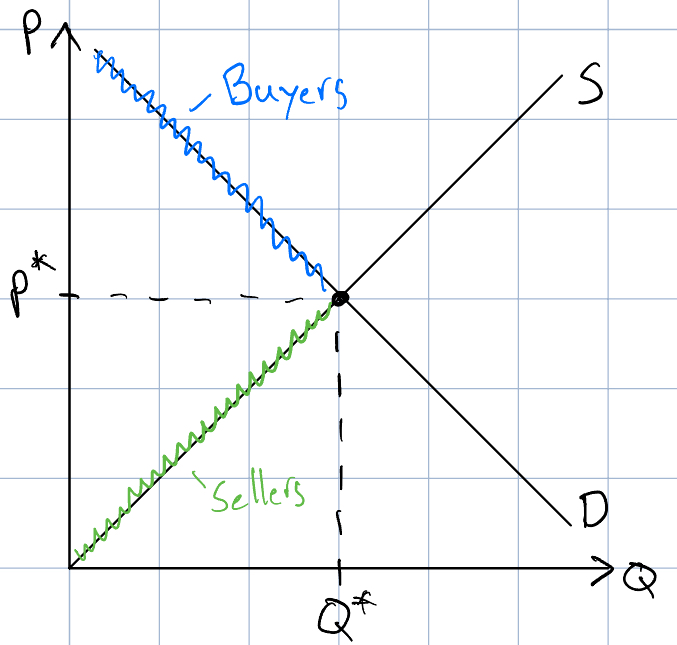
\includegraphics[width = 0.5\textwidth]{qq7}
	\end{center}
	
\item (c) -- At a quantity to the right of equilibrium, the demand curve is below the supply curve. That mean's the marginal buyer's willingness to pay is less than the marginal seller's cost to produce.

\end{enumerate}

\subsection*{Problems and Application}

\begin{enumerate}
\setcounter{enumi}{5}

\item

	\begin{enumerate}
	
	\item 
		\begin{tabular}{c | c | c}
		$P$ & $Q_S$ & $Q_D$ \\
		\hline
		2 & 1 & 3 \\
		4 & 2 & 2 \\
		6 & 3 & 1 \\
		\end{tabular}
		
		A price of \$4 brings supply and demand to equilibrium.
		
	\item From part (b) of \#4 and \#5, we know $CS = 4$ and $PS = 4$. Therefore, $TS = 4 + 4 = 8$.
	
	\newpage
	
	\item Total surplus would decrease to $3 + 3 = 6$.
	
		\begin{center}
		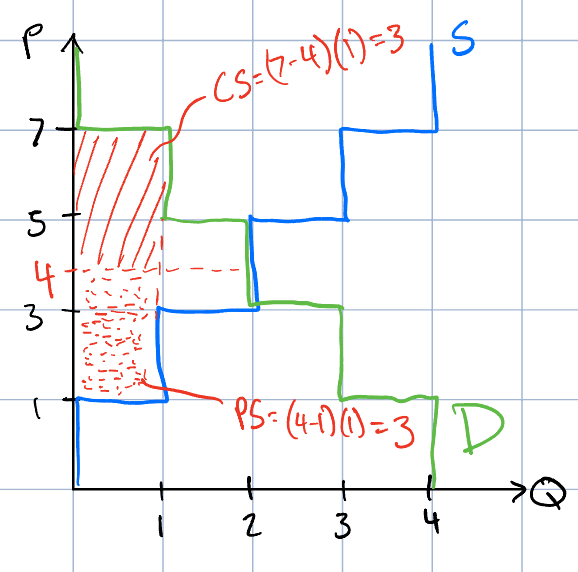
\includegraphics[width = 0.5\textwidth]{paa6c}
		\end{center} 
		
	\item Total surplus would decrease to $8 - 1 - 1 = 6$.
	
		\begin{center}
		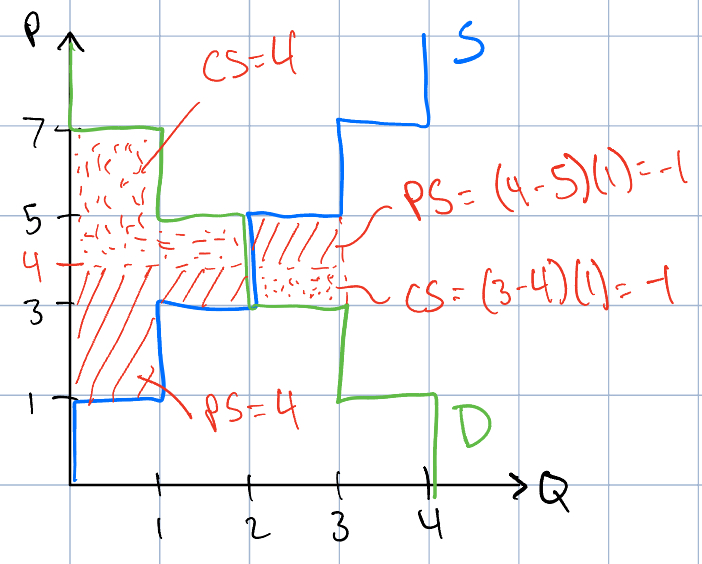
\includegraphics[width = 0.5\textwidth]{paa6d}
		\end{center}
	
	\end{enumerate}
	
\newpage
	
\item

	\begin{enumerate}
	
	\item Supply shifts out in response to falling production costs, so price decreases, and quantity increases. See graph in (b).

	\item Both $CS$ and $PS$ increase.

		\begin{center}
		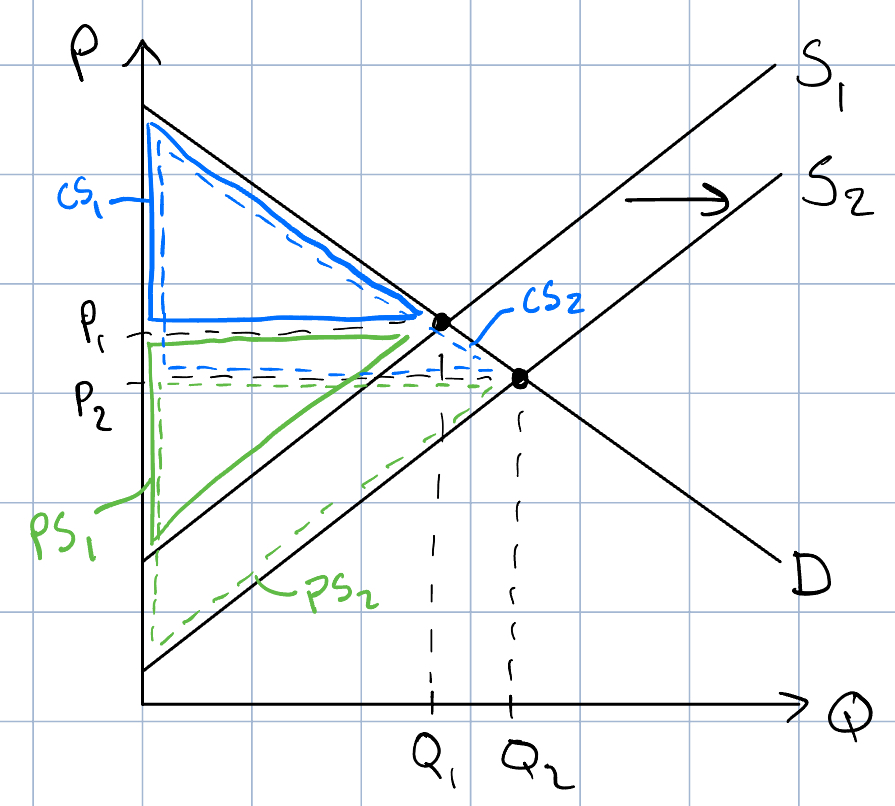
\includegraphics[width = 0.5\textwidth]{paa7ab}
		\end{center}
		
	\item Consumers would benefit most because consumer surplus increases more than producer surplus decreases. 
	
		\begin{center}
		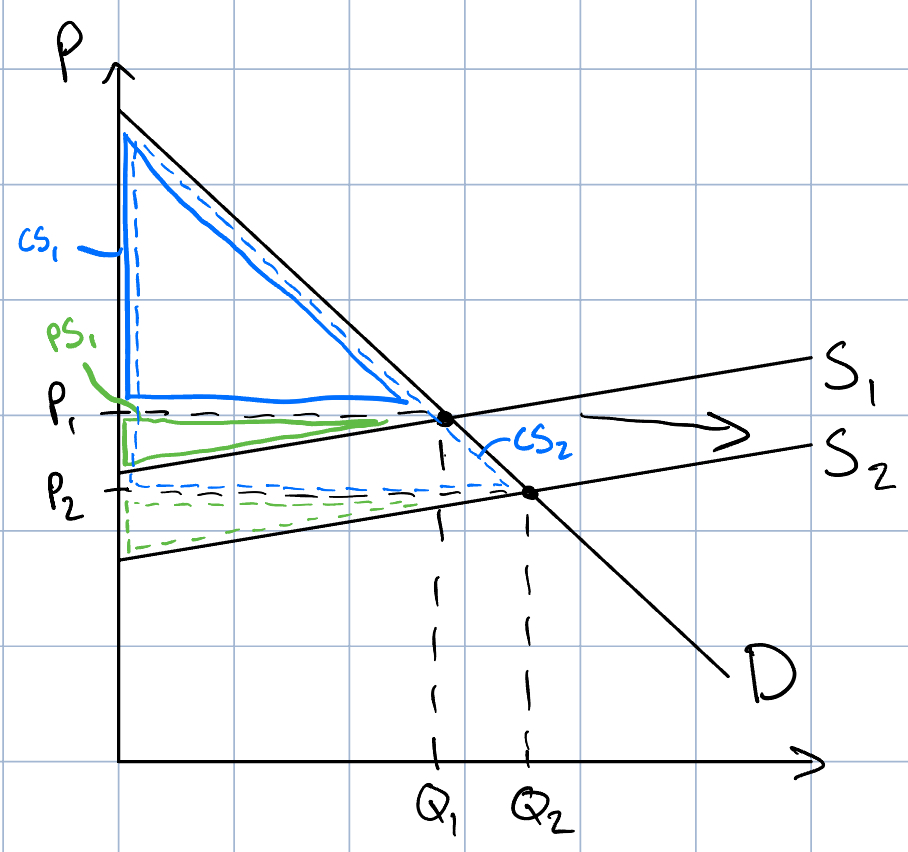
\includegraphics[width = 0.5\textwidth]{paa7c}
		\end{center}
	
	\end{enumerate}
	
\item There should be three haircuts given for a maximum of \$55 in total surplus. The first haircut should go to the person who values it the most and come from the firm that can produce it for the lowest cost. That means Claire should buy a haircut from Firm D which generates $\$40 - \$10 = \$30$ of total surplus. The second haircut should go to the person who values it the second most and come from the firm that can produce it for the second lowest cost. That means Gloria should buy a haircut from Firm B which generates $\$35 - \$15 = \$20$ of total surplus. The third haircut should go to the person who values it the third most and come from the firm that can produce it for the third lowest cost. That means Phil should buy a haircut from Firm C which generates $\$25 - \$20 = \$5$ of total surplus. After that, the marginal buyer, Jay, values a haircut less than it costs the marginal seller, Firm B, to provide the service, so no more haircuts should happen. In this scenario, total surplus is $\$30 + \$20 + \$5 = \$55$. 

\end{enumerate}

\end{document}